%%%%%%%%%%%%%%%%%%%%%%%%%%%%%%%%%%%%%%%%%%%
% Ovdje napisite naziv treceg Sectiona
\Section{Tre\'{c}i naslov} \label{Sec:3}
%
% Ispod napisite tekst Sectiona

% Na primjer
\begin{tm}[Pappusov teorem \cite{PJRyan+EaNEG}]
Neka su e i f dva pravca koji le\v{z}e u projektivnoj ravnini. Neka su A, B i C to\v{c}ke koje le\v{z}e
na pravcu $e$, razli\v{c}ite od to\v{c}ke $e \cap f$ i neka su $A'$, $B'$ i $C'$ tri to\v{c}ke pravca $f$
razli\v{c}ite od to\v{c}ke $e \cap f$. Tada su to\v{c}ke $Q=AB' \cap A'B$, $R=BC' \cap B'C$ i
$S=CA' \cap C'A$ kolinearne.
\end{tm}
%
\begin{figure}[!ht]
\begin{center}
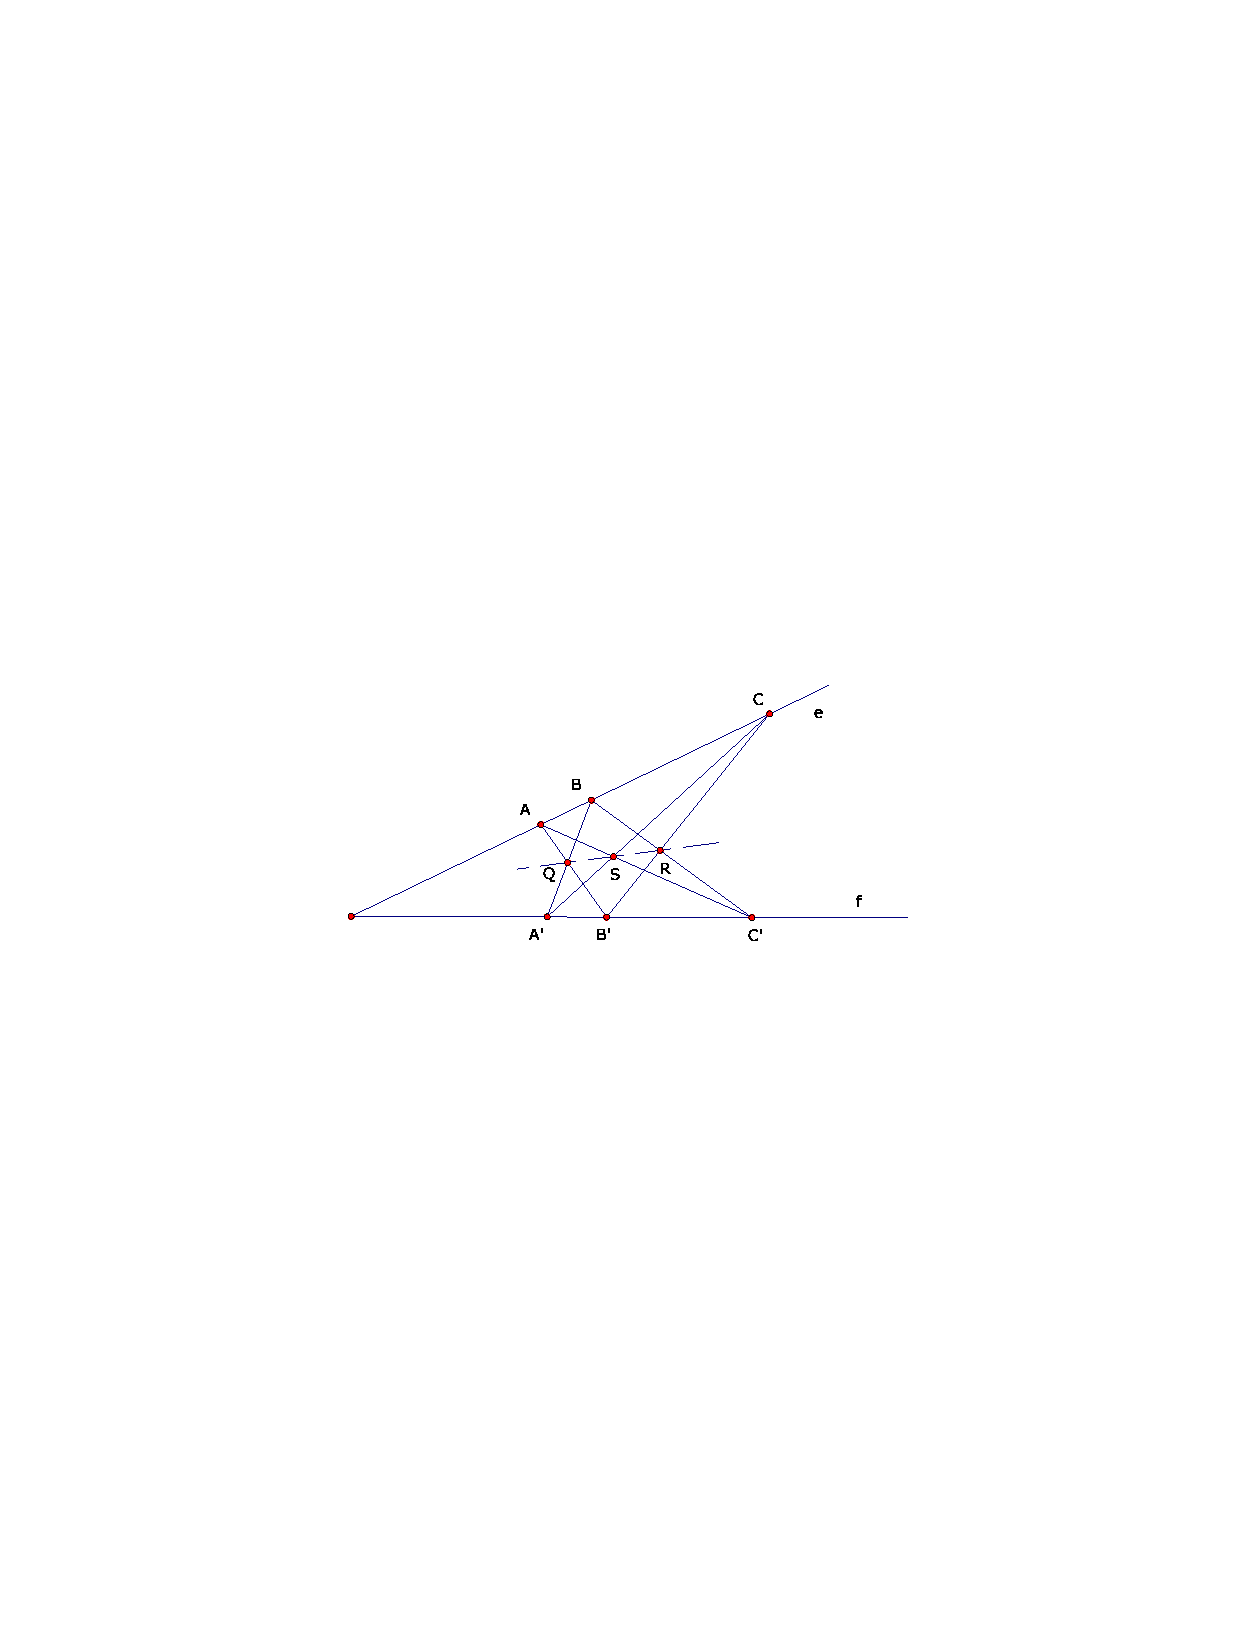
\includegraphics[clip, viewport=150 320 440 460]{slike/slika_3-1.eps}
\caption{}
\label{fig:3.1}
\end{center}
\end{figure}

